%%%%%%%%%%%%%%%%%%%%%%%%%%%%%%%%%%%%%%%%%%%%%%%%%%%%%%%%%%
%%
%% MARK: Title
%%
%%%%%%%%%%%%%%%%%%%%%%%%%%%%%%%%%%%%%%%%%%%%%%%%%%%%%%%%%%

\chapter*{\S B27. The Diffeomorphisms of the Wire Plane}
\setcounter{footnote}{0}

%%%%%%%%%%%%%%%%%%%%%%%%%%%%%%%%%%%%%%%%%%%%%%%%%%%%%%%%%%
%%
%% MARK: Abstract
%%
%%%%%%%%%%%%%%%%%%%%%%%%%%%%%%%%%%%%%%%%%%%%%%%%%%%%%%%%%%

\begin{abstract}
  We prove that the group of diffeomorphisms of the Wire Plane $\cW$
  is identical as a set to the standard diffeomorphism group $\Diff(\RR^2)$,
  yet the two groups are distinct as diffeological groups.
  This completes the Boman Paradox:
  two spaces with the same topology and the same abstract diffeomorphism group
  can be geometrically distinct.
\end{abstract}

%%%%%%%%%%%%%%%%%%%%%%%%%%%%%%%%%%%%%%%%%%%%%%%%%%%%%%%%%%
%%
%% MARK: Introduction
%%
%%%%%%%%%%%%%%%%%%%%%%%%%%%%%%%%%%%%%%%%%%%%%%%%%%%%%%%%%%

In the previous chapter (B26),
we introduced the Wire Plane $\cW$,
a diffeological space with underlying set $\RR^2$ whose plots are those smooth parametrizations that factor locally through smooth curves.
We proved that the D-topology of $\cW$ coincides with the standard Euclidean topology,
yet the diffeological dimension of $\cW$ is $1$, not $2$.

In this chapter,
we complete the paradox by examining the group of diffeomorphisms of $\cW$.
We will show that $\Diff(\cW)$ and $\Diff(\RR^2)$ are identical as sets,
but distinct as diffeological groups.
Thus,
two spaces with the same underlying set,
the same topology,
and the same abstract group of symmetries
can nevertheless be geometrically distinct.

%%%%%%%%%%%%%%%%%%%%%%%%%%%%%%%%%%%%%%%%%%%%%%%%%%%%%%%%%%
%%
%% MARK: Boman's Theorem
%%
%%%%%%%%%%%%%%%%%%%%%%%%%%%%%%%%%%%%%%%%%%%%%%%%%%%%%%%%%%
\section{Boman's Theorem}

The key analytic fact underlying the algebraic identity is a classical theorem of J. Boman \cite{Bom67}.

\textbf{Theorem} (Boman, 1967)
\label{thm:boman}
{\it A function $f: \RR^n \to \RR^m$ is smooth (of class $C^\infty$) if and only if it maps smooth curves to smooth curves.
That is,
for every smooth curve $\gamma: \RR \to \RR^n$,
the composition $f \circ \gamma: \RR \to \RR^m$ is smooth.
}

In other words,
differentiability along all smooth curves suffices to guarantee full smoothness.
This theorem is the engine that will allow us to identify the diffeomorphism groups as sets.

%%%%%%%%%%%%%%%%%%%%%%%%%%%%%%%%%%%%%%%%%%%%%%%%%%%%%%%%%%
%%
%% MARK: Equality of the Groups as Sets
%%
%%%%%%%%%%%%%%%%%%%%%%%%%%%%%%%%%%%%%%%%%%%%%%%%%%%%%%%%%%
\section{Equality of the groups as sets}

We denote by $\Diff(\RR^2)$ the group of standard diffeomorphisms of the plane,
and by $\Diff(\cW)$ the group of diffeomorphisms of the Wire Plane
(bijections $\phi: \RR^2 \to \RR^2$ such that $\phi$ and $\phi^{-1}$ send plots of $\cW$ to plots of $\cW$).

\begin{Article}{Equality as sets}{}
  \label{prop:group-equality}
  As sets,
  $$%
    \Diff(\cW) = \Diff(\RR^2).
    $$%
  That is,
  every standard diffeomorphism of $\RR^2$ is a diffeomorphism of $\cW$,
  and conversely,
  every diffeomorphism of $\cW$ is a standard diffeomorphism.
\end{Article}

\begin{proof}
  We prove the two inclusions separately.
  
  \textbf{1.} $\Diff(\RR^2) \subseteq \Diff(\cW)$.
  
  Let $\phi \in \Diff(\RR^2)$ be a standard diffeomorphism.
  Let $P: U \to \cW$ be a plot of $\cW$.
  By definition of the wire diffeology,
  for every $u \in U$ there exists a neighborhood $V$,
  a smooth curve $\gamma: \RR \to \RR^2$,
  and a smooth function $q: V \to \RR$ such that $P|_V = \gamma \circ q$.
  Then
  $$%
    \phi \circ P|_V = \phi \circ \gamma \circ q.
    $$%
  Since $\phi$ is smooth,
  $\gamma' = \phi \circ \gamma$ is a smooth curve.
  Hence $\phi \circ P$ factors locally through the smooth curve $\gamma'$,
  and is therefore a plot of $\cW$.
  The same argument applies to $\phi^{-1}$.
  Thus $\phi \in \Diff(\cW)$.
  
  \textbf{2.} $\Diff(\cW) \subseteq \Diff(\RR^2)$.
  
  Let $\phi \in \Diff(\cW)$.
  By definition,
  $\phi$ sends plots of $\cW$ to plots of $\cW$.
  In particular,
  for every smooth curve $\gamma: \RR \to \RR^2$,
  which is a plot of $\cW$,
  the composition $\phi \circ \gamma$ is also a plot of $\cW$,
  hence a smooth curve.
  Thus $\phi$ maps smooth curves to smooth curves.
  By Boman's Theorem (Theorem \ref{thm:boman}),
  $\phi$ is smooth in the standard sense.
  The same argument applied to $\phi^{-1}$ shows that $\phi^{-1}$ is also standard smooth.
  Therefore $\phi \in \Diff(\RR^2)$.
\end{proof}

Thus,
as abstract groups,
$\Diff(\cW)$ and $\Diff(\RR^2)$ are indistinguishable.
The paradox deepens.

%%%%%%%%%%%%%%%%%%%%%%%%%%%%%%%%%%%%%%%%%%%%%%%%%%%%%%%%%%
%%
%% MARK: The Groups are Distinct as Diffeological Groups
%%
%%%%%%%%%%%%%%%%%%%%%%%%%%%%%%%%%%%%%%%%%%%%%%%%%%%%%%%%%%
\section{The groups are distinct as diffeological groups}

Although $\Diff(\cW)$ and $\Diff(\RR^2)$ coincide as sets,
they carry different diffeologies.
We equip each group with its \emph{functional diffeology}:
a parametrization $P: U \to \Diff(X)$ is a plot if and only if the evaluation map
$(u,x) \mapsto P(u)(x)$ is smooth from $U \times X$ to $X$
\cite[\textsection\,1.57 and 1.61]{PIZ13}.

Let $j: \Diff(\RR^2) \to \Diff(\cW)$ be the identity map on the underlying set.
We will show that $j$ is not smooth.
Consequently,
the two diffeological groups are distinct.

\begin{Article}{The identity map is not smooth}{}
  \label{prop:non-smooth}
  The identity map $j: \Diff(\RR^2) \to \Diff(\cW)$ is not smooth.
  In particular,
  $\Diff(\cW)$ carries a strictly finer diffeology than $\Diff(\RR^2)$.
\end{Article}

\begin{proof}
  Consider the path of translations $P: \RR \to \Diff(\RR^2)$ defined by
  $$%
    P(t)(x,y) = (x + t, y).
    $$%
  This is a smooth path (a $1$-plot) in the functional diffeology of $\Diff(\RR^2)$,
  because the evaluation map
  $$%
    (t,x,y) \mapsto (x+t, y)
    $$%
  is smooth from $\RR \times \RR^2$ to $\RR^2$.
  
  To test whether $P$ is also a plot of $\Diff(\cW)$,
  we must check if the associated evaluation map
  $$%
    \Eval_P: \RR \times \cW \to \cW,\qquad \Eval_P(t, (x,y)) = (x+t, y)
    $$%
  is smooth as a map of diffeological spaces.
  By definition of the wire diffeology,
  a map into $\cW$ is smooth if and only if it sends plots of the domain to plots of $\cW$.
  
  Consider the plot $Q: \RR^2 \to \RR \times \cW$ defined by
  $$%
    Q(u,v) = (u, (0,v)).
    $$%
  Note that $v \mapsto (0,v)$ is a plot of $\cW$ (it is a smooth vertical line),
  and $u \mapsto u$ is smooth,
  so $Q$ is a plot of the product $\RR \times \cW$.
  
  The composition $\Eval_P \circ Q: \RR^2 \to \cW$ is
  $$%
    \Eval_P(Q(u,v)) = P(u)(0,v) = (u, v).
    $$%
  This is the identity map on $\RR^2$.
  But as we saw in Example 2 of B26,
  the identity map is \emph{not} a plot of $\cW$,
  because it cannot be factored locally through a smooth curve
  (its image contains an open subset of $\RR^2$, which is $2$-dimensional).
  
  Therefore,
  $\Eval_P$ is not smooth,
  and consequently $P$ is not a plot of $\Diff(\cW)$.
  Hence the identity map $j: \Diff(\RR^2) \to \Diff(\cW)$ fails to send a smooth path to a smooth path,
  and is not smooth.
\end{proof}

Thus,
while $\Diff(\cW)$ and $\Diff(\RR^2)$ are identical as abstract groups,
they are distinct as diffeological groups.
The diffeology of $\Diff(\cW)$ is strictly finer:
it admits fewer smooth paths.

%%%%%%%%%%%%%%%%%%%%%%%%%%%%%%%%%%%%%%%%%%%%%%%%%%%%%%%%%%
%%
%% MARK: Completion of the Paradox
%%
%%%%%%%%%%%%%%%%%%%%%%%%%%%%%%%%%%%%%%%%%%%%%%%%%%%%%%%%%%
\section{Completion of the paradox}

We have now established all the pieces of the Boman Paradox.

\begin{Article}{The Boman Paradox}{}
  The standard Euclidean plane $\RR^2$ and the Wire Plane $\cW$ satisfy:
  \begin{enumerate}
    \item They have the same underlying set $\RR^2$.
    \item They have the same D-topology (the Euclidean topology).
    \item They have the same abstract diffeomorphism group $\Diff(\RR^2) = \Diff(\cW)$.
    \item Yet they are geometrically distinct:
    \begin{itemize}
      \item[(a)] $\dim(\RR^2) = 2$ while $\dim(\cW) = 1$.
      \item[(b)] $\Diff(\RR^2)$ and $\Diff(\cW)$ are distinct as diffeological groups.
    \end{itemize}
  \end{enumerate}
  Hence,
  topology together with the abstract group of symmetries
  does not determine the geometry.
\end{Article}

This result forces a refinement of the Kleinian--Souriau perspective.
While the group of diffeomorphisms is a powerful invariant,
it does not capture the full geometric structure.
The missing ingredient is the \emph{local smooth structure},
encoded in the diffeology itself,
which precedes the group and cannot be recovered from it.

The arrow of definition is irreversible:
the space determines the group,
but the group---even as a diffeological group---does not determine the space.

%%%%%%%%%%%%%%%%%%%%%%%%%%%%%%%%%%%%%%%%%%%%%%%%%%%%%%%%%%
%%
%% MARK: Conclusion
%%
%%%%%%%%%%%%%%%%%%%%%%%%%%%%%%%%%%%%%%%%%%%%%%%%%%%%%%%%%%
\section{Conclusion}

The Boman Paradox reveals a fundamental limitation of the radical Kleinian--Souriau program.
While Souriau famously claimed that ``le groupe est la géométrie,''
the Wire Plane $\cW$ shows that two spaces can share the same topology,
the same abstract diffeomorphism group,
yet remain geometrically distinct.

Diffeology,
the very tool Souriau developed to give infinite-dimensional groups a smooth structure,
provides the language in which this distinction becomes visible.
The paradox is not a failure of diffeology,
but a demonstration of its power:
it distinguishes spaces that classical topology and abstract algebra cannot separate.

The moral is clear:
geometry is not reducible to the sum of Topology and Algebra.
It requires a third ingredient:
the local smooth structure,
captured by the diffeology,
which determines the rigidity of the space and the nature of its symmetries.

\vfill
\centerline{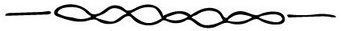
\includegraphics[width=.5\textwidth]{Figures/separator-2.jpg}}
\vfill
